\documentclass[10pt, letterpaper]{article}

% \usepackage{fullpage} % this makes 1 inch margin on all side 
\usepackage[margin=1in]{geometry} % 1 in margin on all sides
\usepackage{tikz, pgfplots}
\usepackage{graphicx}
\usepackage{float}
% \usepackage[top=1in, bottom=1in, left=0.75in, right=0.75in]{geometry} % 1 in margin on all sides
% \usepackage[top=1in, bottom=1in, left=0.75in, right=0.75in, paperwidth=5in, paperheight=7in]{geometry} % 1 in margin on all sides
\usepackage{amsfonts, amssymb, amsmath}
\def\eq1{y=\dfrac{x}{x^{2}+3x+2}}

\newcommand{\set}[1]{\setlength\itemsep{#1em}}

\pgfplotsset{compat=1.16} % this is for compatibility issue
% below makes a command "calculator" using which we get a small calculator font. Currently not working due to some error in code.
% \newcommand\calculator{
% 	\tikz{
% 		\node (c) [inner sep=0pt, draw, fill=black, anchor=south west]{\phantom{N}};
% 		\begin{scope}[x=(c.south east), y=(c.north west)] 
% 			\fill[white](.1, .7) rectangle(.9, .9);
% 			\foreach \x in {.3, .33, .55, .79}{
% 				\foreach \y in {.1, .24, .38, .53}{
% 					\fill[white](\x, \y) rectangle +(.11, .07);
% 				}
% 			}
% 		\end{scope}
% 	}
% }
% \def\calcicon#1{\noindent#1\calculator\}

\begin{document}

\set{5}

\textbf{Critical Thinking Questions}

\begin{center}
% 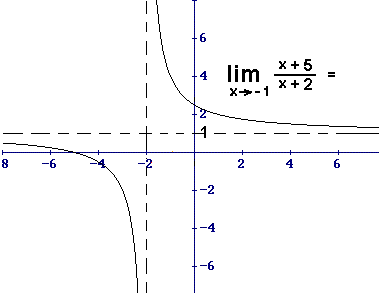
\includegraphics[scale=1]{limit}
% 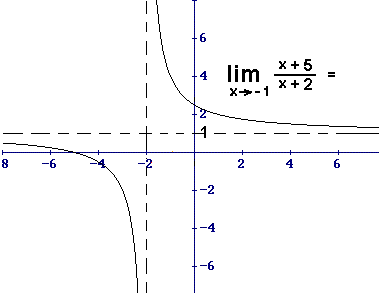
\includegraphics[width=0.5in]{limit}
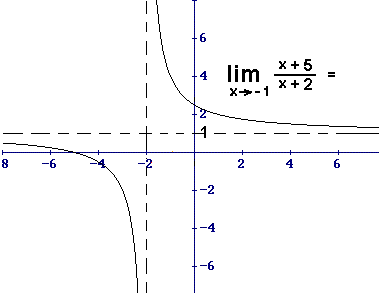
\includegraphics[width=0.4\textwidth]{limit}
\end{center}

\begin{figure}[H] % h for here else it will place according to itself
\centering % to center image and caption
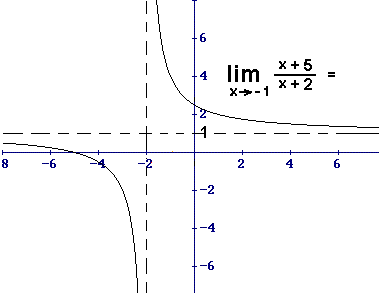
\includegraphics[width=0.4\textwidth]{limit}
\caption{Limit Limit Limit}
\end{figure}

\begin{enumerate}
% \item \calculator Let's examine the equation $\eq1$.
\item Let's examine the equation $\eq1$.
\item This is the symbol for set of real numbers: $\mathbb{R}$
\item This is the symbol for set of integers: $\mathbb{Z}$
\item This is the symbol for set of rationals: $\mathbb{Q}$
\item Is it possible for a sequence to converge to two different numbers? If so, give an example. If not, explain why not? 
\item Explain how to use partial sums to determine if a series converges or diverges.
\item Explain why $ \int \limits_{1}^{\infty} f(x) \, dx $ and $ \sum \limits_{n=1}^{\infty} a_n $ need not to converge to same value even if they are both convergent.
\item In your words explain the Alternating Series Remainder Theorm. How is this theorm useful?
\end{enumerate}


\end{document}
